\section{Organisation de l'équipe}
	\subsection{Équipe de direction}
	L’équipe de direction du projet est composée de nos meilleurs experts dans le domaine de la TMA. 

	Celle-ci est composée de M. Gérard \bsc{Dugalle} et Mme. Lucie \bsc{Rouerg}. Afin de respecter la méthode Kanban, le \textit{Product Owner} sera responsable de la bonne mise en œuvre des attentes du client.
	
	\subsection{Équipe de développement}
	Dans le respect de la méthode agile Kanban, nous avons organisé en notre équipe sous la forme suivante:
	
	\begin{description}
		\item[Product owner]  Il sera chargé de faire avancer le projet dans le sens des besoins de cette TMA.
		\item[Coach Agile]  Il permettra de faire en sorte que les processus de la méthode Kanban soient bien mis en œuvre. 
		\item[Équipe de développement] Elle est en charge d’effectuer les tâches de développement pour répondre aux besoins de la TMA. Cette équipe sera aussi chargée de réaliser l’étude de la TMA ainsi que l’assistance technique. 		
	\end{description}
		
\begin{figure}[H]
\centering
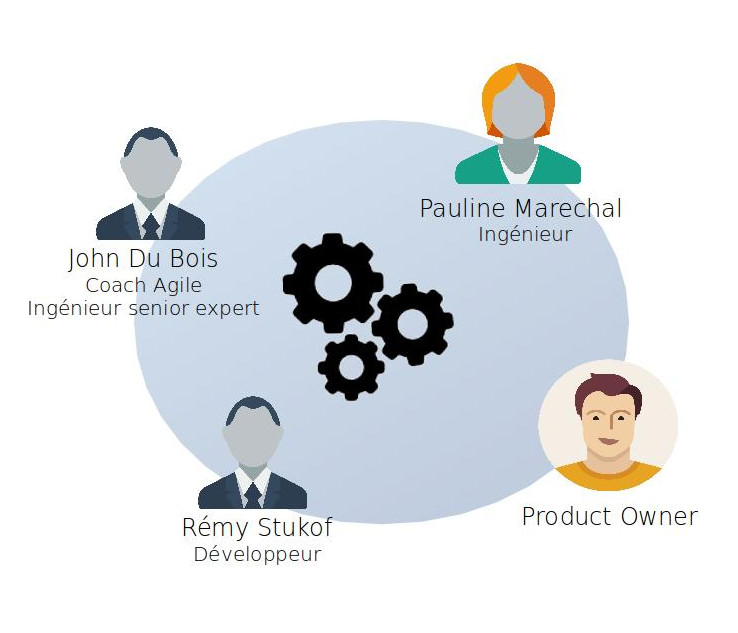
\includegraphics[width=0.7\linewidth]{images/chap2/team}
\caption{L'équipe de développement}
\label{fig:team}
\end{figure}
\subsubsection{Rémy \bsc{Stukof}}
Un jeune développeur passionné des technologies Web. Il a travaillé sur plusieurs de nos projets application JEE / Web sur lesquels il a pu prouver ses compétences en développement web. Rémy est intervenu en tant que renfort sur un certain nombre de nos projets. Il sait ainsi s’adapter à un grand nombre de situations et a l’habitude d’effectuer des opérations de maintenance corrective (correction de bogues) et évolutive. Rémy \bsc{Stukof} aidera Pauline \bsc{Marechal}, dans l’assistance technique en cas de surgissement de bogues. Rémy n’est pas incorporé en temps que membre permanent dans d’autres équipes de développement, ce qui lui donne l’avantage de se rendre immédiatement disponible en cas de besoin sur cette TMA. Rémy travaillera donc à temps plein ou à temps partiel en fonction du besoin et de la charge de travail induite par la TMA. 

\subsubsection{Pauline \bsc{Marechal}}
Un ingénieur possédant de solides compétences en développement sur des technologies très variées. Pauline sera la développeur principale sur les opérations de maintenances évolutives. Elle sera assistée par Rémy. Son expérience permettra de choisir les meilleures solutions et de les mettre en oeuvre avec efficacité. 

\subsubsection{John Du \bsc{Bois}}
Un ingénieur senior qui pourra apporter une aide de haute qualité pour la résolution de problèmes techniques difficiles. Son expérience dans la gestion de projet et de processus lui permettra aussi de s’occuper de ces aspects sur la TMA. Il sera chargé en particulier de contrôler que le processus Kanban est bien respecté et appliqué. Pour des maintenances évolutives d’envergure, son expérience permettra d’approuver ou d’infirmer les architectures proposées et de partager son expertise en développement logiciel. Les spécifications et conceptions qu’il apportera permettront de fournir les lignes directrices et les architectures nécessaires aux développeurs du projet. Son expérience sera aussi sollicitée pour la résolution de bogues difficiles. 

\subsection{Organisation de l'équipe}
Cette équipe sera affectée au projet de manière définitive. Notre politique qualité en matière de méthodes agiles est de pérenniser les équipes de développement en leur donnant les moyens nécessaires. Pour cela un espace de travail commun est mis à leur disposition afin de bien pouvoir mettre en place le processus agile qui demande des interactions. Des outils informatiques communs sont aussi mis à disposition comme décrit dans le chapitre « Plateforme Logicielles». Enfin, le projet est affecté à leur charge de travail et les membres de la conduite opérationnelle ont pour devoir de vérifier que leur charge de travail leur permettant d’assurer toujours à 100\% le besoin du projet. Une fois sélectionnées nos équipes agiles sont amenées à changer qu’en cas de situations exceptionnelles. Enfin, au minimum un créneau horaire hebdomadaire est réservé au \textit{product owner}. Selon les disponibilités du client, il pourra évidemment être élargi. Nos infrastructures permettent aussi la disponibilité à tout moment d’un poste de travail au sein de l’équipe de développement agile pour le \textit{product owner}, même dans le cas où il n’est pas déporté en permanence dans notre entreprise.  